\documentclass[11pt]{article}
\usepackage[letterpaper,margin=1in]{geometry}
\usepackage{color}
\usepackage[dvipdfmx]{graphicx}
\usepackage{amsbsy}
\usepackage{amsmath}
\usepackage{adjustbox}
\usepackage{url}
%\usepackage{floatrow}
\usepackage[font=small,labelfont=bf,tableposition=top]{caption}
\DeclareCaptionLabelFormat{tableonly}{\tablename~\thetable}
%\newfloatcommand{capbtabbox}{table}[][\FBwidth]


\newcommand{\argmax}{\mathop{\rm arg~max}\limits}

\begin{document}
\vspace{-1cm}
\title{\vspace{-2ex}Analysis Report on Assignment 2: Logistic Regression\vspace{-2ex}}
\author{Yoshinari Fujinuma\vspace{-2ex}}
\date{\vspace{-2ex}}
\maketitle

%How did the learning rate affect the convergence of your SGA implementation?
%What was your stopping criterion and how many passes over the data did you need to complete before stopping?
%What words are the best predictors of each class? How (mathematically) did you find them?
%What words are the poorest predictors of classes? How (mathematically) did you find them?

%\section{The relationship between the learning rate and convergence}
\vspace{-0.5cm}
%The following two graph shows the relationship between training examples and accuracy:
\begin{figure}[htb]
  %\vspace{-1.1cm}
  \begin{center}
   \begin{tabular}{c}
    \begin{minipage}{0.5\hsize}
     %\vspace{-0.5cm}
     \begin{center}
     %\scalebox{0.25}
     \scalebox{0.33}
      %{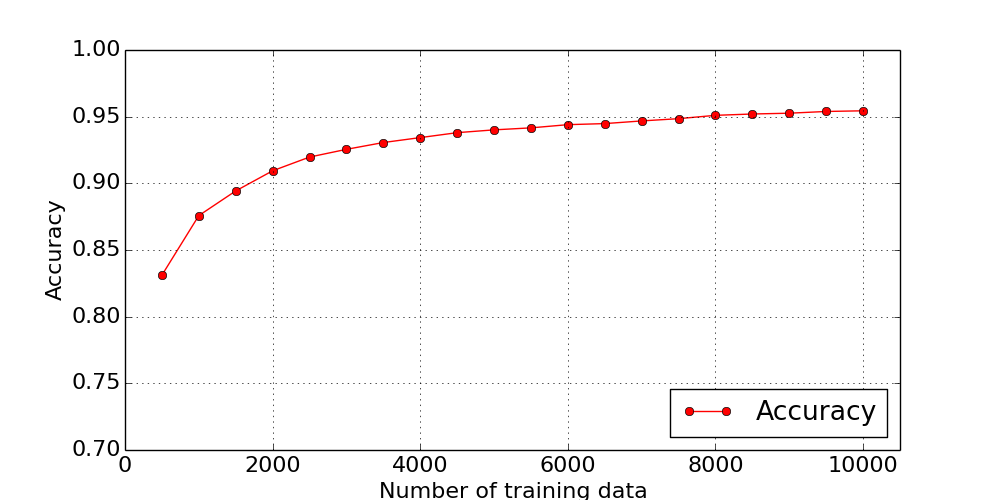
\includegraphics[]{figure_1.png}}
      {\includegraphics[]{figure_1_updated.png}}
   
      \caption{The accuracy of hold out test dataset. The value of $passes$ is fixed to $1$. }
      \label{fig:learning_rate}
     \end{center}
    \end{minipage}

    \begin{minipage}{0.01\hsize}
    \end{minipage}

    \begin{minipage}{0.5\hsize}
     \begin{center}
      \scalebox{0.33}
      {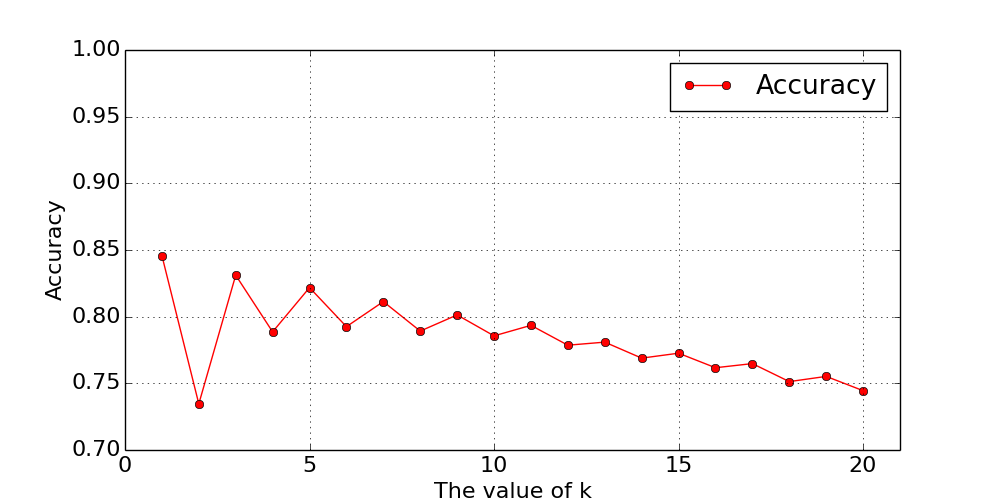
\includegraphics[]{figure_2.png}}
      \caption{\label{stopping_criterion}Stopping criterion.}
     \end{center}
    \end{minipage}

  \end{tabular}
 \end{center}
\vspace{-0.5cm}
\end{figure}

According to Figure \ref{fig:learning_rate}, the smaller the learning rate is, it converges faster. 
%After the update $5641$ the hold out accuaracy only takes four values which ranges between $0.92$ and $0.95$. 
When the hold out accuracy remains same through 100 updates, I used that as a stopping criterion. In fact, the hold out accuracy from Update 2151 through 2251 did not change as shown in Figure \ref{stopping_criterion}.

%\section{Best and Worst Contributing Words}
\begin{table*}[h]
 \begin{minipage}{.33\linewidth}
  \centering
  \begin{tabular}{|l|l|r|r|r|r|}
  \hline \bf Word     & \bf Weight     \\ \hline
  hit      & $1.62$ \\
  pitching & $1.40$ \\
  baseball & $1.30$ \\
  runs     & $1.27$ \\
  better   & $1.09$  \\
  \hline
  \end{tabular}
 \caption{\label{positive_class} The top $5$ weighted words for the baseball class. }
 \end{minipage}
 \begin{minipage}{.33\linewidth}
  \centering
  \begin{tabular}{|l|l|r|r|r|r|}
  \hline \bf Word     & \bf Weight     \\ \hline
  pts      & $-6.29$ \\
  period   & $-2.29$ \\
  hockey   & $-2.24$ \\
  vs       & $-2.12$ \\
  shots    & $-1.99$ \\
  \hline
  \end{tabular}
 \caption{\label{negative_class} The top $5$ weighted words for the hockey class. }
 \end{minipage}
 \begin{minipage}{.33\linewidth}
  \centering
  \begin{tabular}{|l|l|r|r|r|r|}
  \hline 
%\bf Word     & \bf Weight     \\ \hline
  aggravatingly       & favour         \\
  alway               & pronunciation  \\
  baby                & prototypical   \\
  contained           & ratio          \\
  crumbled            & sportscasters  \\
  \hline
  \end{tabular}
 \caption{\label{neutral_class} List of words with $0$ weights. }
 \end{minipage}

%\vspace{-0.5cm}
%\caption{\label{_result} Learned weights of each word.}
\end{table*}

The best predictors for the baseball class and the hockey class are shown in Table \ref{positive_class} and Table \ref{negative_class} respectively. These words are found by sorting the words by its learned weights and get the lowest $5$ words and the highest $5$ words. The worst predictors are shown in Table \ref{neutral_class}.

\begin{figure}[htb]
  \begin{center}
   \begin{tabular}{c}
    \begin{minipage}{0.5\hsize}
     \vspace{-0.3cm}
     \begin{center}
     %\scalebox{0.33}
     \scalebox{0.25}
      {\includegraphics[]{figure_3.png}}
   
      \caption{The learning curve for scheduled vs. non-scheduled learning rates. }
      \label{fig:eta}
     \end{center}
    \end{minipage}

    \begin{minipage}{0.01\hsize}
    \end{minipage}

 \begin{minipage}{.33\linewidth}
  \centering
  \begin{tabular}{|l|l|r|r|r|r|}
  \hline 
  \bf Without tfidf     & \bf With tfidf     \\ \hline
   pts           & attendance  \\
   period        & shots  \\
   hockey        & period  \\
   vs            & pp  \\
   shots         & pts  \\
  \hline
  \end{tabular}
    \captionlistentry[table]{A table beside a figure}
    \captionsetup{labelformat=tableonly}
    \caption{\label{tfidf}The top weighted words for predicting hockey class.}
 \end{minipage}
%    \begin{minipage}{0.5\hsize}
%     \begin{center}
%      \scalebox{0.33}
%      {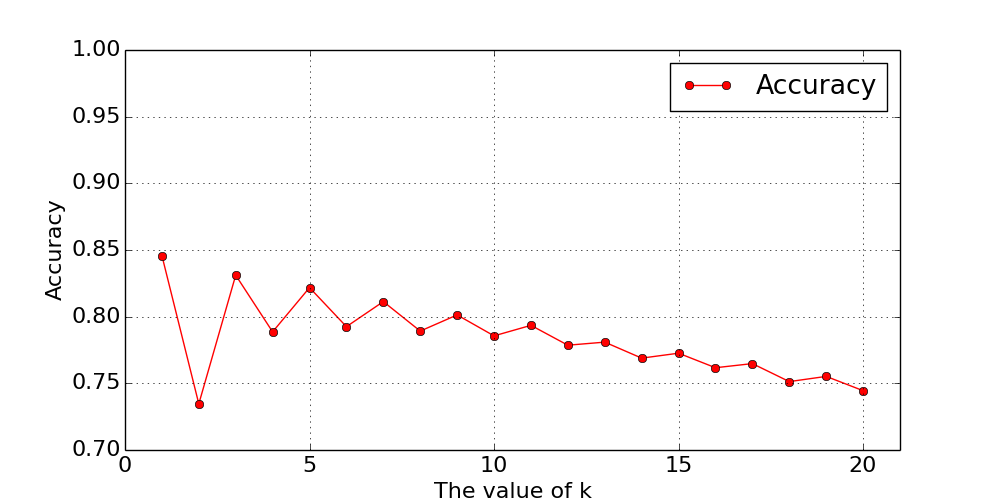
\includegraphics[]{figure_2.png}}
%      \caption{\label{stopping_criterion}Stopping criterion.}
%     \end{center}
%    \end{minipage}

  \end{tabular}
 \end{center}
\vspace{-0.5cm}
\end{figure}

%\begin{figure}[h]
%\begin{floatrow}
%\ffigbox{%
%      {\includegraphics[]{figure_3.png}}
%}{%
%  \caption{A figure}%
%}
%\killfloatstyle
%\ttabox{%
%%\capbtabbox{%
%  \begin{tabular}{cc} \hline
%  Author & Title \\ \hline
%  Knuth & The \TeX book \      Lamport & \LaTeX \\ \hline
%  \end{tabular}
%}{%
%  \caption{A table}%
%}
%\end{floatrow}
%\end{figure}

As shown in Figure \ref{fig:eta}, by implementing a learning rate that gradually decreases, it converges faster than the one without schedule. Table \ref{tfidf} shows the result of with and without using tfidf as a feature. Tfidf helps weigh less on common words such as ``vs''. Note that the actual weight on the word ``hockey'' increased even though it does not show up in Table \ref{tfidf} after using the tfidf feature.

\end{document}
